\subsection{Team 1}
\label{app:team1}

\paragraph{Data} Segmentation training used the 2,992 ReXGroundingCT
training scans with their findings and masks. The image encoder, CIRCLE, was
pretrained on 403,500 non-contrast chest CT scans from 288,740
patients, paired with radiology reports. Additional in-house data comprised
950 scans from the CIRCLE cohort at Zhongshan Hospital, Fudan University,
Shanghai, China: 800 scans with pulmonary nodules and 150 challenging
scans covering lung cancer, pneumonia and other infections, and less common
thoracic conditions. Positive finding descriptions were extracted from each
report, and annotation engineers with medical backgrounds exhaustively
delineated every visible abnormality corresponding to each finding, yielding
paired descriptions and 3D masks. No test-set images or text were used at any
stage, including the pretraining of components.

\paragraph{Pre-processing} Volumes were resampled to
0.65 $\times$ 0.65 $\times$ 1.15\,mm, with an input size of
384 $\times$ 320 $\times$ 224 voxels.

\paragraph{Architecture and text encoder} CIRCLE pretraining jointly learns
image--report alignment and abnormality recognition. A 3D adaptation of
EfficientNetV2-XL \citep{tan2021efficientnetv2} and a Chinese BERT-based report
encoder project CT volumes and reports into a shared 512-dimensional space. A
SigLIP-style contrastive objective \citep{zhai2023sigmoid} aligns
image--report pairs, while a parallel classification head predicts 37 thoracic
abnormalities from report-derived labels with binary cross-entropy. For
grounding, the pretrained image encoder was integrated into VoxTell
\citep{rokuss2026voxtell} (Figure~\ref{fig:app-team1}): a prompt decoder
conditions segmentation on features from a frozen Qwen3-Embedding-4B text encoder
\citep{zhang2025qwen3}, and the image encoder and segmentation decoder are
fine-tuned.

\paragraph{Training} Dice plus binary cross-entropy loss, AdamW with an initial
learning rate of $3 \times 10^{-4}$, and a batch size of 24. Training took about
two days on eight H20 GPUs.

\paragraph{Ensembling} Probability maps from checkpoints of different epochs
were averaged voxel-wise.

\paragraph{Post-processing} The averaged probability map was thresholded at
0.5. No other post-processing was applied.

\paragraph{Inference time and hardware} About 20\,s per scan per finding on one
H20 GPU.

\paragraph{Final submission and lessons} The final submission is listed as
``CIRCLE'' on the leaderboard. On a 50-case validation subset, pretraining
raised mean Dice from 0.277 with random initialization to 0.327,
against 0.282 for VoxTell, and the in-house data raised it further to
0.356. Pretraining and additional annotations therefore helped, whereas the
same architecture trained from scratch did not improve on VoxTell.

\paragraph{Code and weights} Code: \url{https://github.com/uii-open-source/CIRCLE/}.
Model weights are not publicly released.

\begin{figure}[!htbp]
\centering
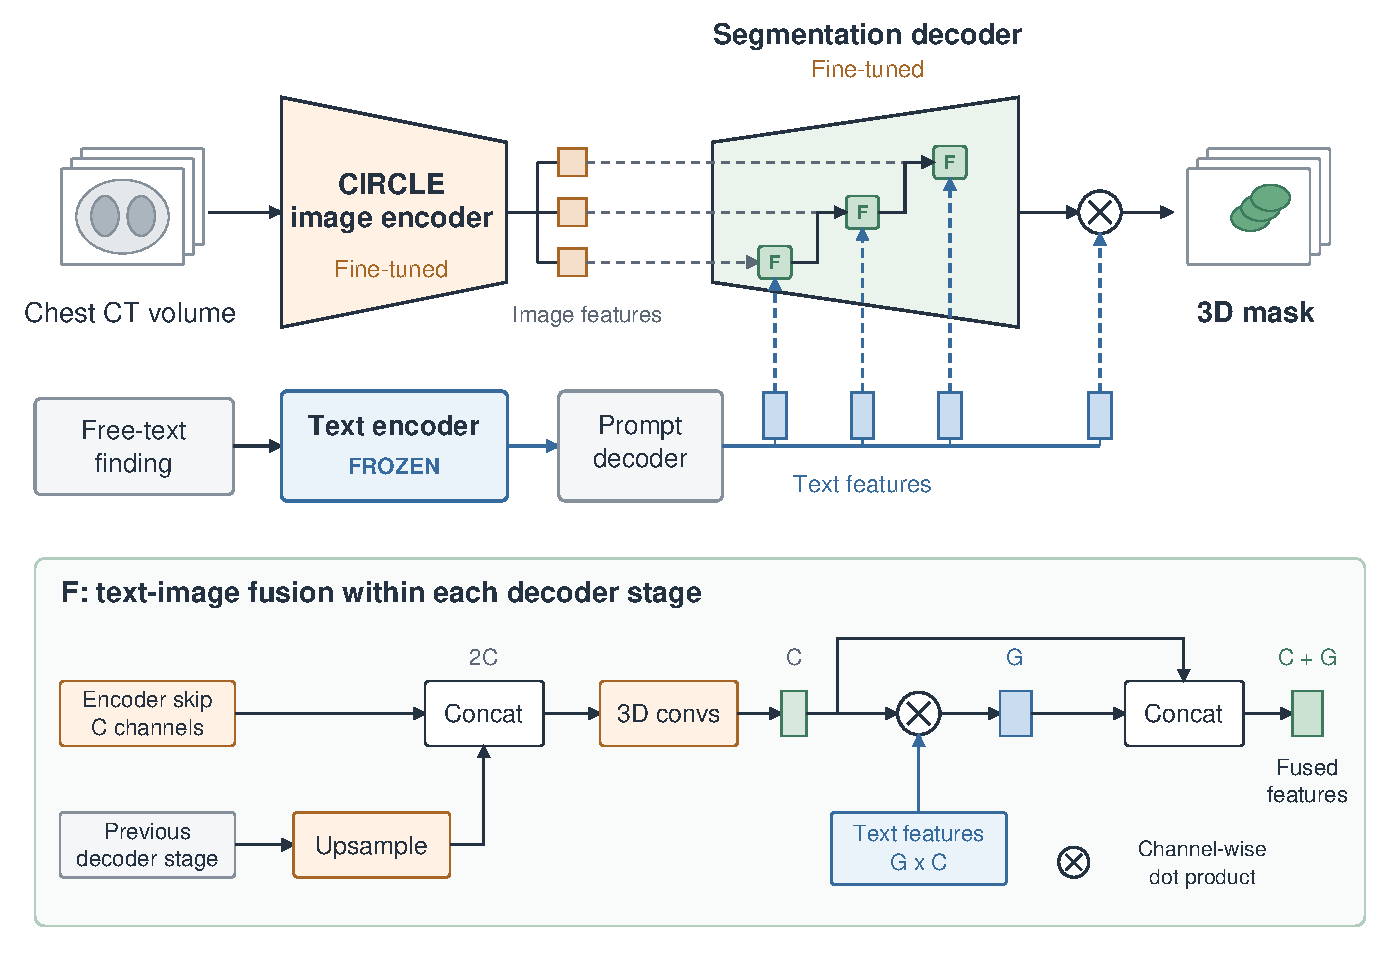
\includegraphics[width=\columnwidth]{figures/appendix/team1_pipeline.pdf}
\caption{Team 1: the pretrained CIRCLE image encoder combined with a VoxTell-based
decoder. The image encoder and segmentation decoder are fine-tuned, and the text
encoder is frozen. Inset F shows the text--image fusion within each decoder
stage.}
\label{fig:app-team1}
\end{figure}
